\documentclass[10pt,a4paper]{article}
\usepackage[utf8]{inputenc}
\usepackage{amsmath}
\usepackage{amsfonts}
\usepackage{amssymb}
\usepackage{graphicx}
\usepackage{tikz}
\usetikzlibrary{positioning}

\DeclareMathOperator{\conv}{conv}

\newtheorem{observation}{Observation}

\begin{document}
	\section{Trivial example 1}
	Consider the graph
\begin{center}
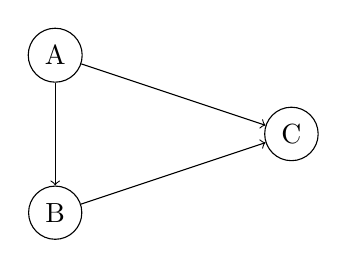
\begin{tikzpicture}
	\node[shape=circle,draw=black] (A) at (0,1) {A};
	\node[shape=circle,draw=black] (B) at (0,-1) {B};
	\node[shape=circle,draw=black] (C) at (3,0) {C};
	\draw[->] (A) edge (B);
	\draw[->] (A) edge (C);
	\draw[->] (B) edge (C);
	%\draw[color=gray] (0,0) -. (C);
\end{tikzpicture}
\end{center}
where $A$ is located at $(0,1)$, $B$ is located at $(0,-1)$ and $C$ is located at $(h,0)$. Denote the distance from $A$ or $B$ to $C$ by $l$. The supplies are $s_A = (1,0)$, $s_B = (0,1)$ and $s_C = (-1,-1)$. Consider the trivial cost function $c(x,y) = |x+y|$ where $x, y$ are the amounts of (signed) flow. Then
\[
\partial c(0,0) = \conv\left\{ (1,1),(-1,-1),(1,-1),(-1,1) \right\}
\]
or with inequalities $\partial c(0,0) = \{z:\, |e_i^T z| \leq 1 \,\forall i \}$. Obviously, an optimal flow is
\begin{align*}
f = \begin{pmatrix}
1&0\\0&1\\0&0
\end{pmatrix}.
\end{align*}
An optimal dual solution is $\phi_A = (l,l)$, $\phi_B = (l,l)$ and $\phi_C = (0,0)$. It can be easily checked that this satisfies all constraints. The derivative of $\phi$ is
\[
D\phi = \begin{pmatrix}
-l/h & 0\\-l/h & 0
\end{pmatrix}.
\]
We now check whether $D\phi$ meets the constraints, i.e. if $\lVert e_i^T D\phi \rVert\leq 1$. We see that $\lVert e_i^TD\phi \rVert = l/h > 1$ for all $i$. This is maybe surprising, as the flow $f$ is globally optimal (with respect to all possible graph topologies).
\begin{observation}
	Even if the global optimum is found, the dual constraints might not be satisfied.
\end{observation}
Since $e_i^T D\phi = (-l/h,0)$, this suggests that we should add an edge parallel to $(1,0)$ to the graph.
\end{document}